\documentclass[12pt, titlepage, a4paper]{article}
\usepackage[utf8]{inputenc}
\usepackage{changepage}
\usepackage{prftree}
\usepackage{amssymb}
\usepackage{amsmath}
\usepackage{enumitem} 
\usepackage{graphicx}
\usepackage{wrapfig}
\usepackage[spanish]{babel}
\usepackage{amsthm}
\usepackage{bussproofs}
\usepackage{bm}
\usepackage{url}
\usepackage{hyperref}

\usepackage[edges]{forest}
\definecolor{folderbg}{RGB}{165, 105, 189}
\definecolor{folderborder}{RGB}{165, 105, 189}
\newlength\Size
\setlength\Size{4pt}
\tikzset{%
  folder/.pic={%
    \filldraw [draw=folderborder, top color=folderbg!50, bottom color=folderbg] (-1.05*\Size,0.2\Size+5pt) rectangle ++(.75*\Size,-0.2\Size-5pt);
    \filldraw [draw=folderborder, top color=folderbg!50, bottom color=folderbg] (-1.15*\Size,-\Size) rectangle (1.15*\Size,\Size);
  },
  file/.pic={%
    \filldraw [draw=folderborder, top color=folderbg!5, bottom color=folderbg!10] (-\Size,.4*\Size+5pt) coordinate (a) |- (\Size,-1.2*\Size) coordinate (b) -- ++(0,1.6*\Size) coordinate (c) -- ++(-5pt,5pt) coordinate (d) -- cycle (d) |- (c) ;
  },
}
\forestset{%
  declare autowrapped toks={pic me}{},
  pic dir tree/.style={%
    for tree={%
      folder,
      font=\ttfamily,
      grow'=0,
    },
    before typesetting nodes={%
      for tree={%
        edge label+/.option={pic me},
      },
    },
  },
  pic me set/.code n args=2{%
    \forestset{%
      #1/.style={%
        inner xsep=2\Size,
        pic me={pic {#2}},
      }
    }
  },
  pic me set={directory}{folder},
  pic me set={file}{file},
}

\usepackage{listings}

\usepackage{blindtext}
\usepackage[a4paper, total={6in, 8in}]{geometry}

\title{Trabajo Practico Final \\ 
Análisis del Lenguaje de Programación \\
Sistema F}
\author{Ramiro Gatto}
\date{.../.../2025}

\begin{document}
\maketitle

\section{Descripción del Proyecto}
La idea principal del proyecto es la de implementar un EDSL sobre el Sistema F, el cual permita la evaluación de algunos términos del mismo. Para  
que el proyecto sea simple se eligieron un par de tipos bases para el evaluador, los cuales son: 
\begin{itemize}[label=$\bullet$]
    \item {Empty}
    \item {Booleanos}
    \item {Naturales}
    \item {Funciones}
    \item {Listas (de cualquier tipo)}
\end{itemize}

\noindent Además, para el evaluador también se definió lo siguiente:
\begin{itemize}[label=$\bullet$]
    \item {Chequeador de tipos}
    \item {Pretty-printer}
    \item {Parser}
\end{itemize}

Para poder realizar el mismo se tomo como inspiración el Trabajo Practico Nº2 \cite{tp2:lambdaCalculoSimpleTipado}, el cual se 
extendió/modifico para satisfacer con lo requerido.


\section{Manual de uso e Instalación del software}
Para poder usar el evaluador se va a necesita de Stack \cite{haskellStack}, una vez instalado se tiene que abrir una consola en el 
directorio del proyecto (Sistema-F) y ejecutar:
\begin{enumerate}
    \item stack setup (una única vez)
    \item stack build
    \item stack exec Sistema-F-exe
\end{enumerate}

\noindent Con las dos primeras lineas compilamos el proyecto y con la tercera lo ejecutamos.

% Agregar un poco mas

\section{Organización de los archivos}
\noindent La organización de los archivos del proyecto es la siguiente:

\begin{forest}
    pic dir tree,
    where level=0{}{
      directory,
    },
  [Sistema-F
    [.stack-work]
    [app
     [Main.hs, file]
    ]
    [dist-newstyle]
    [src
     [Common.hs, file]
     [Parse.y, file]
     [PrettyPrinter.hs, file]
     [SystamF.hs, file]
    ]
    [.gitignore, file]
    [CHANGELOG.md, file]
    [Ejemplos.txt, file]
    [LICENSE, file]
    [package.yaml, file]
    [README.md, file]
    [Sistema-F.cabal, file]
    [stack.yaml, file]
    [stack.yaml.lock, file]
  ]
\end{forest}


Para entender el como funciona el proyecto veamos la función de los archivos en las carpetas app y src que son los principales para 
el funcionamiento del mismo, el resto de los archivos son de configuración.

\subsection{app}
\subsubsection{Main.hs}
Este archivo es donde comienza la ejecución del programa al compilarse y ejecutarse (implementa el ejecutable final). Hace uso de una 
serie de funciones para poder parser la entrada por teclado, determinar el comando ingresado, imprimir por pantalla, realizar la evaluación, entre muchas cosas más.

\subsection{src}
\subsubsection{Common.hs}
En este archivo es donde se encuentran las definición de los tipo y valores. Es decir es donde se definen los términos y valores que utilizara el Sistema F.

\subsubsection{Parse.y}
Para generar el parser utilizaremos happy. En este archivo se generan los parsers a utilizar, se definen los tokens que acepta el parse, 
entre más funciones. También es donde se define el lexer que se utilizara como analizador lexicográfico de la entrada. \\ 

Para crear el archivo se utilizo el Parser.y del TPº2 \cite{tp2:lambdaCalculoSimpleTipado} y la documentación de Happy \cite{haskellHappy}.

\subsubsection{PrettyPrinter.hs}
Para poder mostrar los términos se utilizo la biblioteca pretty printing, la cual consiste en una serie de combinados desarrollada por John Hughes. Aca es 
donde se encuentra implementado el pretty printer para el Sistema F. \\
Aca podemos distinguir 2 función importantes:
\begin{itemize}[label=$\bullet$]
  \item {pp: la cual dado un Term lo imprime por pantalla.}
  \item {printType: la cual se encarga de imprimir por pantalla los Type}
\end{itemize}

\subsubsection{SystamF.hs}
En este archivo es donde se implementan las funciones de evaluación y el chequeador de tipo (además de unas cuantas funciones auxiliares).

\section{Decisiones de diseño importantes}
\subsection{Representación del Sistema F}
\noindent Los tipos, valores y términos en el Sistema F están dados por la siguientes gramática:
\begin{align*}
    T &::= E \mid T \rightarrow T \mid X \mid \forall X \ . \ T \mid Bool \mid Nat \mid List \ T\\
    v &::= True \mid False \mid nv \mid \lambda x:T. \ t \mid \Lambda X \ . \ t \\
    nv &:: = 0 \mid suc \ nv \\
    t &::= x \mid \lambda x:T. \ t \mid t \ t \mid ifthenelse \ t \ t \ t \mid \Lambda X \ . \ t \mid t \ \langle X \rangle \\
\end{align*}

Como se menciono anteriormente, la implementación de estos se encuentra en el archivo \textbf{src/Common.hs} y es la siguiente:

\noindent Para los tipos es:
\begin{verbatim}
    data Type = EmptyT 
              | ListTEmpty
              | FunT Type Type
              | BoundForAll Int
              | VarT String
              | ForAllT Type
              | BoolT
              | NatT
              | ListT Type
              deriving (Show, Eq)
\end{verbatim}

De este definición podemos ver que hay más elementos en Type que en la gramática de tipos, esto se debe a que se agregaron 2 tipos más
los cuales son BoundForAll y ListEmpty. \\

Como se van a poder usar listas de todo tipo surge un problema a la hora de usar una lista vacía, ya que se debería especificar el tipo, 
a pesar de estar vacía. 
Para evitar y simplificar esto lo que decidió fue darle un tipo especial a la lista vacía \textbf{ListTEmpty}, de esta forma se evita 
tener que darle un tipo especifico.

Pero esto trajo problemas, por ejemplo en la función infer' en el caso de RL o en la función match en el caso de compara el tipo de una lista vacía con un tipo que es 
una lista pero no vacía. Para solucionar este inconveniente lo que se hizo fue separar en casos, uno es cuando la lista es 
vacía y el otro cuando no es una lista vacía.\\

En el caso del BoundForAll, este no es un tipo per se, sino que su función es similar a la idea 
de los indices de De Brujin. Esto seria, coloquialmente hablando, indicar a que \textbf{para todo} esta ligada la variable cuantificada, la idea es la siguiente:

\begin{center}
    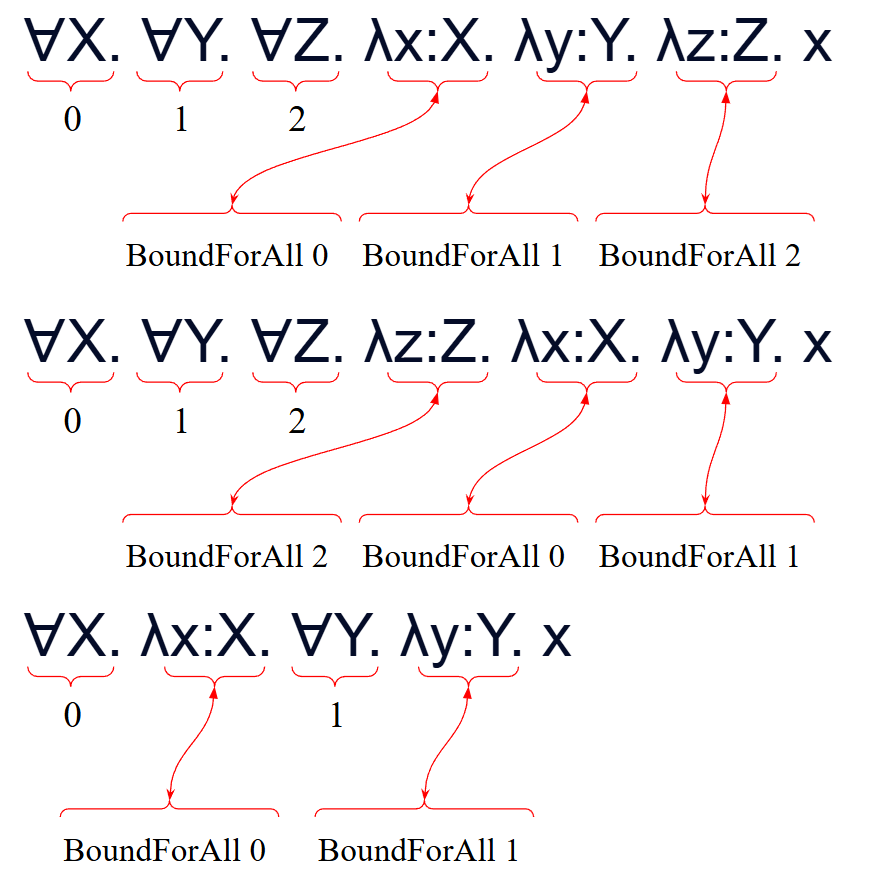
\includegraphics[width=0.7\textwidth]{Imagenes/EjemploBoundForAll.png}
\end{center}

En un inicio la idea era poner el BoundForAll con los Term (como el Bound que esta en Term), pero como esta idea esta relacionada con 
los tipos resulto más practico agregarlo aca.

\noindent Para las expresiones del lambda calculo se tiene:
\begin{verbatim}
    data LamTerm  =  LVar String
                  |  LAbs String Type LamTerm
                  |  LApp LamTerm LamTerm
                  |  LTAbs String LamTerm
                  |  LTApp LamTerm Type
                  |  LTrue 
                  |  LFalse
                  |  LIfThenElse LamTerm LamTerm LamTerm
                  |  LZero
                  |  LSuc LamTerm
                  |  LRec LamTerm LamTerm LamTerm
                  |  LNil
                  |  LCons LamTerm LamTerm
                  |  LRecL LamTerm LamTerm LamTerm
                  deriving (Show, Eq)
\end{verbatim}

Al igual que en el Trabajo Practico 2 \cite{tp2:lambdaCalculoSimpleTipado} surge el problema del uso de nombre de variables, al 
momento de realizar operaciones como la sustitución. Para arreglar esto se mantiene la misma idea de 
usar la representación con \textbf{indices de De Brujin}. \\

Al usar una representación sin nombre surge el problema de no tener variables libres,  
para evitar este inconveniente se utiliza la representación localmente sin nombres (donde variables libres y ligadas están 
en diferentes categorías sintácticas). \\

\noindent Al utilizar esta representación los términos quedan asi:
\begin{verbatim}
    data Term  = Bound Int
               | Free Name 
               | Term :@: Term
               | Lam Type Term
               | ForAll Term
               | TApp Term Type
               | T
               | F
               | IfThenElse Term Term Term
               | Zero
               | Suc Term
               | Rec Term Term Term
               | Nil
               | Cons Term Term
               | RecL Term Term Term
            deriving (Show, Eq)
\end{verbatim}

\subsubsection{Evaluación}
Para la evaluación el interprete sigue el orden de reducción \textbf{call-by-value} en donde tenemos las siguientes reglas, las cuales 
son las presentes en el TP Nº2 \cite{tp2:lambdaCalculoSimpleTipado} y el material de clase del Sistema F \cite{ALP:Polimorfismo}:

\begin{displaymath}
    \prftree[r]{(E-App1)}{t_1 \rightarrow t_1'}{t_1 \ t_2 \rightarrow t_1' \ t_2}  \hspace{1cm}
    \prftree[r]{(E-App2)}{t_2 \rightarrow t_2'}{v \ t_2 \rightarrow v \ t_2'}  \hspace{1cm}
    \prftree[r]{(E-AppAbs)}{}{(\lambda x : T_1 \ . \ t_1 ) v \rightarrow t_1[x/v]}
\end{displaymath}

\begin{displaymath}
    \prftree[r]{E-IFTrue}{ifthenelse \ T \ t_2 \ t_3}{t_2} \hspace{0.5cm}
    \prftree[r]{E-IFFalse}{ifthenelse \ F \ t_2 \ t_3}{t_3} \hspace{0.5cm}
\end{displaymath}
\begin{displaymath}
    \prftree[r]{E-IF}{t_1 \rightarrow t_1'}{ifthenelse \ t_1 \ t_2 \ t_3 \rightarrow ifthenelse \ t_1' \ t_2 \ t_3}
\end{displaymath}

\begin{displaymath}
    \prftree[r]{E-RZero}{R \ t_1 \ t_2 \ 0 \rightarrow t_1} \hspace{0.5cm}
    \prftree[r]{E-RSuc}{R \ t_1 \ t_2 (suc \ t) \rightarrow t_2 (R \ t_1 \ t_2 \ t) t} \hspace{0.5cm}
    \prftree[r]{E-R}{t_3 \rightarrow t_3'}{R \ t_1 \ t_2 \ t_3 \rightarrow R \ t_1 \ t_2 \ t_3'}
\end{displaymath}


\begin{displaymath}
    \prftree[r]{E-RNil}{RL \ t_1 \ t_2 \ nil \rightarrow t_1} \hspace{0.5cm}
    \prftree[r]{E-RCons}{RL \ t_1 \ t_2 (cons \ t \ l) \rightarrow t_2 \ t \ l \ (RL \ t_1 \ t_2 \ l)} \hspace{0.5cm}
\end{displaymath}
\begin{displaymath}
    \prftree[r]{E-RL}{t_3 \rightarrow t_3'}{RL \ t_1 \ t_2 \ t_3 \rightarrow RL \ t_1 \ t_2 \ t_3'} \hspace{0.5cm}
\end{displaymath}
\begin{displaymath}
  \prftree[r]{E-Cons1}{t_1 \rightarrow t_1'}{cons \ t_1 \ t_2 \rightarrow cons \ t_1' \ t_2} \hspace{0.5cm}
  \prftree[r]{E-Cons2}{t_2 \rightarrow t_2'}{cons \ t_1 \ t_2 \rightarrow cons \ t_1 \ t_2'} \hspace{0.5cm}
\end{displaymath}


\begin{displaymath}
    \prftree[r]{E-TApp}{t_1 \rightarrow t_1'}{t_1 \ \langle T \rangle \rightarrow t_1' \ \langle T \rangle} \hspace{1cm}
    \prftree[r]{E-TAppAbs}{(\Lambda X \ . \ t)\ \langle T \rangle \rightarrow t[T/X]}
\end{displaymath}

\subsubsection{Tipos}
Para realizar la inferencia de tipo usamos las siguientes reglas, las cuales al igual que en la sección anterior son las
presentes en el TP Nº2 \cite{tp2:lambdaCalculoSimpleTipado} y en el material de clase del Sistema F \cite{ALP:Polimorfismo}:

\begin{displaymath}
    \prftree[r]{T-True}{\Gamma \vdash T: Bool} \hspace{0.5cm}
    \prftree[r]{T-False}{\Gamma \vdash F:  Bool} \hspace{0.5cm}  
    \prftree[r]{T-IF}{\Gamma \vdash t_1 : Bool}{\Gamma \vdash t_2 : T}{\Gamma \vdash t_3 : T}{\Gamma \vdash ifthenelse \ t_1 \ t_2 \ t_3 \ : \ T} \hspace{1cm}
\end{displaymath}

\begin{displaymath}
    \prftree[r]{T-Zero}{\Gamma \vdash 0 : Nat} \hspace{1cm}
    \prftree[r]{T-Suc}{\Gamma \vdash t : Nat}{\Gamma \vdash suc \ t : Nat} \hspace{1cm}
\end{displaymath}
\begin{displaymath}
    \prftree[r]{T-Rec}{\Gamma \vdash t_1 : Nat}{\Gamma \vdash t_2 : T \ \rightarrow \ Nat \rightarrow \ T}{\Gamma \vdash t_3 : Nat}{\Gamma \vdash suc \ R \ t_1 \ t_2 \ t_3 : T} \hspace{1cm}
\end{displaymath}

\begin{displaymath}
    \prftree[r]{T-Nil}{\Gamma \vdash nil : ListEmpty} \hspace{1cm}
    \prftree[r]{T-Cons}{\Gamma \vdash t_1 : T}{\Gamma \vdash t_2 : List \ T}{\Gamma \vdash cons \ t_1 \ t_2 :  List \ T} \hspace{1cm}
\end{displaymath}
\begin{displaymath}
    \prftree[r]{T-RL}{\Gamma \vdash t_1 : T}{\Gamma \vdash t_2 : T_1 \ \rightarrow \ List \ T_1 \rightarrow \ T \rightarrow \ T}{\Gamma \vdash t_3 : List \ T_1}{\Gamma \vdash \ RL \ t_1 \ t_2 \ t_3 \ : \ T} \hspace{1cm}
\end{displaymath}

\begin{displaymath}
    \prftree[r]{T-TAbs}{\Gamma, X \vdash t : T}{\Gamma \vdash \Lambda X \ . \ t : \forall X \ . \ T} \hspace{1cm}
    \prftree[r]{T-TApp}{\Gamma \vdash t_1 : \forall X \ . \ T}{\Gamma \vdash t_1 \langle T_2 \rangle : T[T_2/X]} \hspace{1cm}
\end{displaymath}

\subsection{Mostrar terminos}
Al igual que en el TP Nº2 \cite{tp2:lambdaCalculoSimpleTipado} se va a utilizar la biblioteca \textbf{pretty printing} para mostrar por 
pantalla. En el archivo
\textbf{src/PrettyPrinter.hs} es donde se implementa el \textbf{pretty printing} para el sistema F.

\subsection{Ejmplos con resultados}
Una vez que se haya compilado y ejecutado el programa nos aparecerá en la consola esto:

\begin{verbatim}
Intérprete de Sistema F
Escriba :help para recibir ayuda.
SF>
\end{verbatim}

Luego si se quiere evaluar una expresión del Sistema F, se la ingresa por teclado, se presiona el enter y listo 
(también hay más opciones como el :print para mostrar los ASTs y el :type para ver el tipo de la expresión, entre muchas otras). \\

Veamos ejemplos (estos ejemplos están en el archivo Ejemplos.txt para que puedan ser testeados sin problemas por el lector):

\subsubsection{Funcion identidad polimorfica}
\noindent En el Sistema F se escribiría: $\Lambda X.\ \lambda $x:X$. \ x$ \\
En la consola escribimos: /\textbackslash X. \textbackslash x:X . x \\
Si quisiéramos evaluarla a un natural escribimos: (/\textbackslash X. \textbackslash x:X . x)  $<$Nat$>$ (suc 0) \\
El cual se reduce a: suc 0

\subsubsection{Funcion length para listas polimorfica}
\noindent En el Sistema F se escribiría: $\Lambda X.\ \lambda xs:List \ X. \ $RL 0 $(\lambda $x:X$ \ .$ys:List X$ \ .$r:Nat$\ .suc\ r)\ xs$ \\
En la consola escribimos: (/\textbackslash X. (\textbackslash xs:List X. RL 0 (\textbackslash x:X .\textbackslash ys:List X. \textbackslash r:Nat. suc r) xs)) \\
Si quisiéramos evaluarla a una lista de funciones polimorficas escribimos: 
((/\textbackslash X. (\textbackslash xs:List X. RL 0 (\textbackslash x:X .\textbackslash ys:List X. \textbackslash r:Nat. suc r) xs)) $<$\textbackslash/X. X -$>$ X$>$) 
(cons (/\textbackslash X. \textbackslash x:X. x) cons (/\textbackslash X. \textbackslash x:X. x) nil)\\
El cual se reduce a: suc suc 0 \\

\noindent (Si se prueba con nil da como resultado 0)

\subsubsection{Funcion que toma como argumento una funcion polimorfica}
\noindent En el Sistema F se escribiría: $\Lambda A.\ \lambda a:A.\ \lambda b:(\forall B. B \rightarrow  B). \ b$ \\
En la consola escribimos: (/\textbackslash A. \textbackslash a:A. \textbackslash b:(\textbackslash /B. B -$>$ B) . b)\\
Si quisiéramos evaluarla podria ser algo asi: (((((/\textbackslash A. \textbackslash a:A. \textbackslash b:(\textbackslash /B. B -$>$ B) . b) $<$Nat$>$) 0) (/ \textbackslash X. \textbackslash x:X. x)) $<$Bool$>$) T\\
El cual se reduce a: T


\bibliographystyle{unsrt}
\bibliography{lib}

\end{document}